% !TEX root = ../../main.tex

\section{Measuring the enthalpy of adsorption}

Experimentally, two methods are widely used for determining the
enthalpy of adsorption. The first relies on measurement of two
or more isotherms at different temperatures and the use of
a Clausius-Clapeyron-type equation for indirect calculation,
while the second is a direct measurement of the evolved heat
during adsorption using calorimetry.

A value for the enthalpy of adsorption in a particular system
may also be obtained from computer simulation methods.
The accuracy of these procedures depends on the accuracy of
the chosen model of interaction between simulated species.

\subsection{Isosteric enthalpy of adsorption}

If the differential enthalpy of adsorption is assumed to be independent
of temperature, \autoref{calo:eqn:enthalpy} can be differentiated
with respect to temperature keeping the surface adsorbed amount constant
to obtain an equation analogous to the Clausius-Clapeyron equation:
%
\begin{equation}
	\Big( \frac{\partial \ln p}{\partial T} \Big)_{n_a} = -\frac{\Delta_{ads}\dot{h}_{T, \Gamma}}{R T^2}
\end{equation}
%
The equation can be rearranged to calculate the differential enthalpy:
%
\begin{equation}\label{calo:eqn:claus-clap}
	\Delta_{ads}\dot{h}_{T, \Gamma} = R \Big( \frac{\partial \ln p}{\partial 1 / T} \Big)_{\Gamma}
\end{equation}
%
where \(\Delta_{ads}\dot{h}_{T, \Gamma}\) is the often termed the
isosteric enthalpy of adsorption.

In order to approximate the partial differential, two or more
isotherms are measured at different temperatures. The temperature
range chosen is usually small, to maintain the assumption of invariance
of isosteric enthalpy with temperature while still obtaining good 
separation between the two isotherms.
Afterwards the isosteric enthalpy of adsorption can be calculated
by using the pressures at which the loading is identical using the
rearranged equation. By plotting the values of \(\ln p\) against
\(1 / T\) we should obtain a straight line with a slope
of \(- \Delta_{ads}\dot{h}_{T, \Gamma} / R\).

As experimental isotherms do not necessarily have points spaced
at equal loading intervals, interpolation is usually used to obtain
data at the desired points. Alternatively, a model may be used
to first fit the isotherm, which is then used for the calculation.

The isosteric enthalpy is sensitive to differences in pressure between
the two isotherms. If the isotherms measured are too close together,
the error margin will increase. The method also assumes that isosteric
enthalpy does not vary with temperature. If the
variation is large for the system in question, the calculation will
lead to unrealistic values. Another requirement is that no phase 
changes in either guest or host occur during adsorption. Thus,
the isosteric method is not suited to soft materials, where the
structural changes are often in themselves temperature dependent.

Even with carefully measured experimental data, there are several
assumptions used in applying \autoref{calo:eqn:claus-clap} to
a real system: 
an ideal bulk gas phase and a negligible adsorbed phase
molar volume. These have a significant effect on the calculated
isosteric enthalpy of adsorption, especially at high relative pressures
and for heavy adsorbates.

\subsection{Microcalorimetry}\label{calo:method:calo}

A direct measurement of the enthalpy of adsorption is possible using
calorimetric methods.
An isothermal calorimeter is most often used for this purpose,
to best approximate a reversible exchange of heat between the
system under investigation and the surrounding
heat sink. To allow for a complete integration of evolved heat,
with minimal losses, a 3D Tian-Calvet thermopile~\cite{calvetRecentProgressMicrocalorimetry1963}
can be used. In order to limit variations in environment,
differential mounting is employed, in which the signal
is the difference in voltage between a reference and experimental
thermopile. In order to ensure the ``isothermicity'' of the calorimeter, a
suitable heat sink must be used, leading to two types of design.
Ambient temperature calorimeters use resistance heating to
maintain the internal temperature, while utilising the environment
as its heat sink. At low temperature, the
environment acts as a heat source and therefore the heat sink must
be provided, often in the form of a constant-temperature bath
undergoing a phase change (e.g.\ liquid \ce{N2}, \ce{Ar}) 
or through a cryostat. Sketches of
an ambient and a low temperature differential Tian-Calvet calorimeter
can be seen in \autoref{calo:fig:calo-types}.

\begin{figure}[htb]

	\centering
	\begin{subfigure}[b]{.45\textwidth}
		\centering
		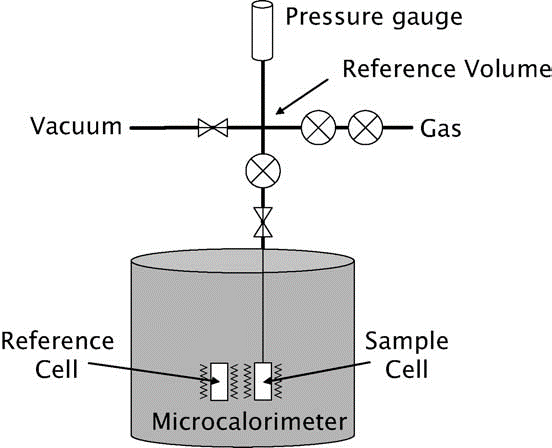
\includegraphics[width=\linewidth]{calo-ht}
		\caption{Ambient-temperature calorimeter}%
		\label{calo:fig:calo-ht}
	\end{subfigure}
	\begin{subfigure}[b]{.5\textwidth}
		\centering
		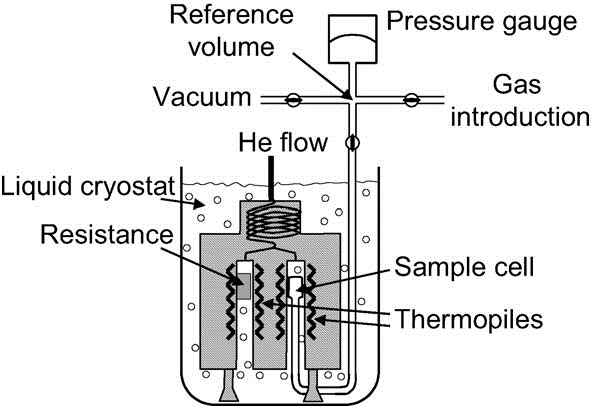
\includegraphics[width=\linewidth]{calo-lt}
		\caption{Low-temperature calorimeter}%
		\label{calo:fig:calo-lt}
	\end{subfigure}%
	\caption{Two types of isothermal Tian-Calvet calorimeters
		for adsorption measurements, specialized for
		different temperature ranges.
		Adapted from \citet{llewellynGasAdsorptionMicrocalorimetry2005}.
	}%
	\label{calo:fig:calo-types}

\end{figure}

Care must be taken to ensure that
the recorded heat through such an experiment can be related directly
to adsorption enthalpy and not to other heat effects.
The adsorbate and gas residing inside a calorimeter is best
represented by an open system, where the introduction of adsorbate
is done through steps that are small enough to consider a reversible
process~\cite{rouquerolGasSolidInteractions1980}.
The accepted convention is that the adsorbate itself is inert and
therefore does not contribute to the variation of any state function.
Under these conditions,
the change in internal energy of the adsorbate can be written as:
%
\begin{equation}
	dU = dQ_{rev} + dW_{rev} + u_T^g dn
\end{equation}
%
where \(dQ_{rev}\) is the reversibly exchanged heat which is
measured by the calorimeter. \(dW_{rev}\) is the reversible work
done by the gas against the external pressure. In the cell volume measured
by the calorimeter (\(V_C\)), this work may be expressed as
%
\begin{equation}
	dW_{rev} = RT dn^{\sigma} + V_C dp
\end{equation}
%
If the previous two equations are combined and differentiated with
respect to the amount adsorbed \(n^{\sigma}\), then we obtain
the equation for the differential heat of adsorption.
%
\begin{equation}
	\frac{dQ_{rev}}{dn^{\sigma}} + V_C \frac{dp}{dn^{\sigma}} = %
	\frac{dU^{\sigma}}{dn^{\sigma}} - u^g - RT = \Delta_{ads}\dot{h}_{T, \Gamma}
\end{equation}

Two options exist regarding the method of introduction of adsorbate:
the continuous and the discontinuous or point-by-point method. In
the point-by-point method, discrete insertion steps are made.
A reference volume is filled with gas at a pressure \(p\), which
is allowed to equilibrate before a valve between the reference volume
and the cell containing the adsorbate is opened, letting the
gas adsorb onto the material. With small enough steps, the
assumption of a reversible system can be approximated.
The peak in the calorimetric signal is integrated over time
to give the total energy released during this adsorption step.

In the other method, the flow of adsorbate is continuous, usually kept
constant by a restriction in the pipe diameter which is severe enough
to allow the gas to enter via sonic flow regimes. At this point, the
flowrate is no longer influenced by a pressure differential,
instead becoming a function only of upstream pressure and environment
temperature.
The heat evolved during adsorption (or required during desorption)
is therefore measured either as discrete peaks, corresponding to
each introduction event or as a continuous heat curve. An example of such a signal
for each method presented in \autoref{calo:fig:calo-measure}.

\begin{figure}[htb]

	\centering
	\begin{subfigure}[b]{.5\textwidth}
		\centering
		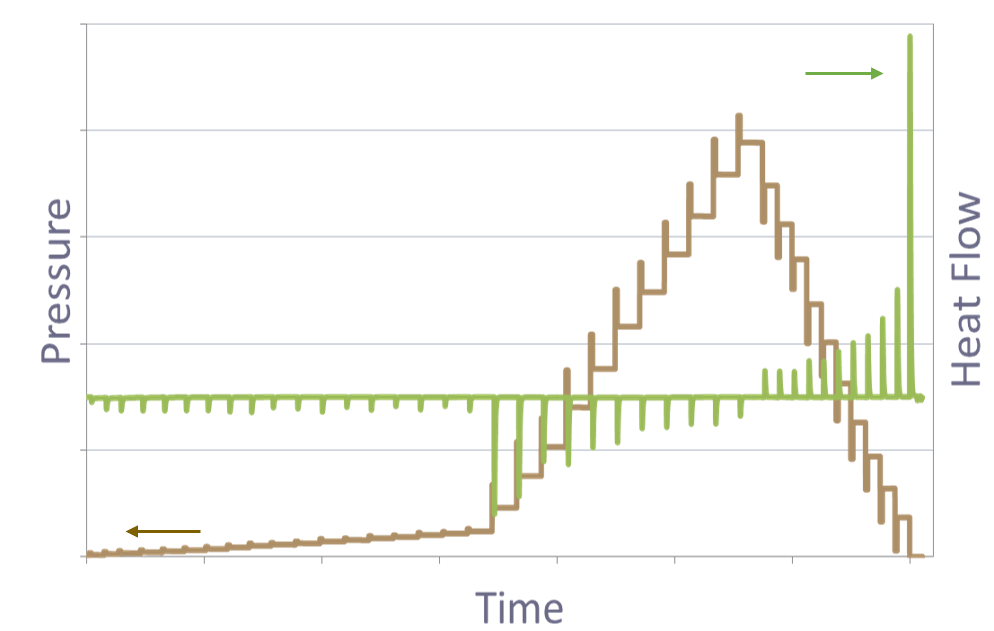
\includegraphics[width=\linewidth]{calo-point}
		\caption{}%
		\label{calo:fig:calo-point}
	\end{subfigure}
	\begin{subfigure}[b]{.48\textwidth}
		\centering
		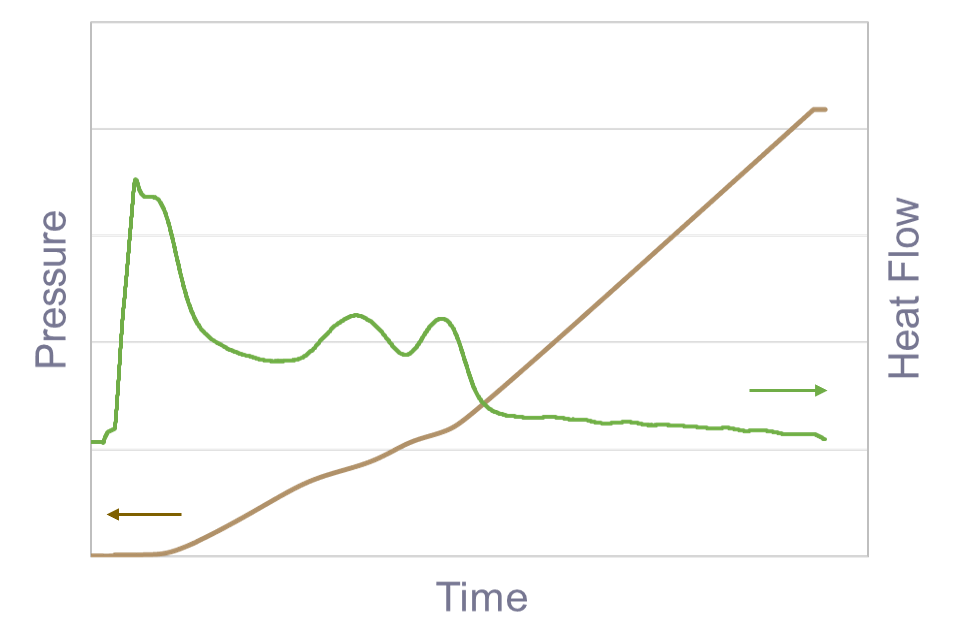
\includegraphics[width=\linewidth]{calo-cont}
		\caption{}%
		\label{calo:fig:calo-cont}
	\end{subfigure}%
	\caption{Typical pressure and calorimeter signals for the two
		available methods of introducing adsorbate into the measurement
		cell (a) discontinuous and (b) continuous.
	}%
	\label{calo:fig:calo-measure}

\end{figure}

The point-by-point method has a lower resolution than
continuous introduction, as the measured heat is necessarily a 
cumulative value of instantaneous
differential enthalpy for the coverage range of each adsorbed point.
However, it has the advantage of ensuring complete equilibrium at
each step, by observing the return to the baseline of the calorimetry
signal or a stable pressure signal. On the other hand, the
continuous method allows for subtle changes in the differential enthalpy of
adsorption, such as those corresponding to adsorbed phase changes,
to be seen experimentally. Additionally, the time-resolved data
can be used to investigate transient phenomena. Equilibrium between
the adsorbed phase and gas phase is no longer guaranteed, and must be
tested for by performing multiple experiments at different adsorbate
flowrates. Alternatively, the experiment can be stopped to observe that the
time for the heat signal to return to its baseline does not diverge
from the dead time of the calorimeter.

\subsection{Experimental apparatus and accuracy}

In this thesis, combined isotherms and enthalpy of adsorption
measurements were made experimentally using a Tian-Calvet type
microcalorimeter coupled with a home-made manometric gas dosing
system~\cite{llewellynGasAdsorptionMicrocalorimetry2005}.
Two calorimeter designs were used, one for ambient temperature
and one for low temperature adsorption, as displayed in
\autoref{calo:fig:calo-types}. 

The method of adsorbate introduction can be chosen either as
continuous or discontinuous. For routine measurements,
the point-by-point method is preferred, as it is guaranteed
to achieve equilibrium between the material and the adsorbate
removing the influence of diffusion effects.
For each injection of gas, equilibrium was assumed to have
been reached after \SIrange{90}{250}{\minute}, depending on the
sample and adsorbate used. This was confirmed by the return
of the calorimetric signal to its baseline (<\SI{5}{\micro\watt}).
For the continuous method, a sonic nozzle was used to 
maintain the flowrate between \SIrange{0.5}{2}{\micro\mol\per\minute},
low enough that the system can be considered at equilibrium. 
The assumption of equilibrium is routinely verified by multiple
experiments at different upstream pressures.

As the isotherms are recorded through the manometric method,
the accuracy in the adsorbed amount depends on the reliability
of measuring individual state variables (temperature,
pressure, volume) and the equation of state relating them 
to adsorbate loading.
Characteristic to this method, the pressure recorded for 
a point is measured in relation to the previous one. Therefore,
the error is cumulative with each successive measurement point,
and is the largest contribution to the total error. The 
uncertainty can be lowered dramatically by increasing 
the available surface area inside the calorimeter.
Between \SIrange{50}{200}{\milli\gram}
of sample is used in each experiment, such that the specific
surface area inside the calorimeter cell is larger than
\SI{50}{\metre^2\per\gram}. Finally, the REFPROP equation
of state is used~\cite{lemmonNISTReferenceFluid1989}, 
currently the most accurate available.
Overall, error in isotherms measured in this way can be 
reduced to less than 5\%.

The error in the differential enthalpy of adsorption has a
contribution from both the heat signal of the calorimeter 
and the accuracy in the amount adsorbed.
At low coverage the error in the calorimetric signal can be
estimated to around \( \pm \) \SI{0.2} {\kilo\joule\per\mol}.
This uncertainty is orders of magnitude lower than the contribution
from loading, and is therefore omitted in the error calculation.
As the value obtained from integration of the signal peaks
must be divided by the change in adsorbed amount \(\Delta n\),
the error is largest in flat sections of the isotherm, where 
the amount adsorbed is low. Thus, uncertainty varies from 
0.5--5\% in the beginning of the isotherm to over 100\% when
an isotherm plateau is reached.

A complete error analysis for the resulting isotherms and enthalpy
curves can be found in \autoref{appx:errors}. Also, a direct comparison
between calorimetry and gravimetry isotherms is presented in the 
following section.